\section*{Lecture 16: Recursion (\textsection 5.6--7)}

We now describe how recurrence relations arise from recursive algorithms,
and begin to look at ways of solving them.
We have just learned one method that can sometimes be used to solve
such a relation, namely Mathematical Induction.
In fact, we can think of recursion as backwards induction.

\begin{definition}[Recurrence Relation]
    A \emph{recursive sequence} $a_0, a_1, a_2, \ldots$ is a sequence such that:
    \begin{itemize}
        \item For small enough $k$, the value of $a_k$ is explicitly specified.
            (called the \emph{initial conditions}).
        \item For large enough $k$, defines $a_k$ in terms of one or more of the
            terms that appear before $a_k$. (called the \emph{recurrence
            relation}).
    \end{itemize}
\end{definition}

For example, the Fibonacci numbers are given by the initial conditions $f_0=0$,
$f_1=1$, and, for all $k \geq 2$, $f_k=f_{k-1}+f_{k-2}$.  What are the first few
Fibonacci numbers?
\practice

Can you prove that for
all $i \geq 2$, $f_i$ is even iff $i$ is odd?

\begin{figure}[tbh]
    \centering
    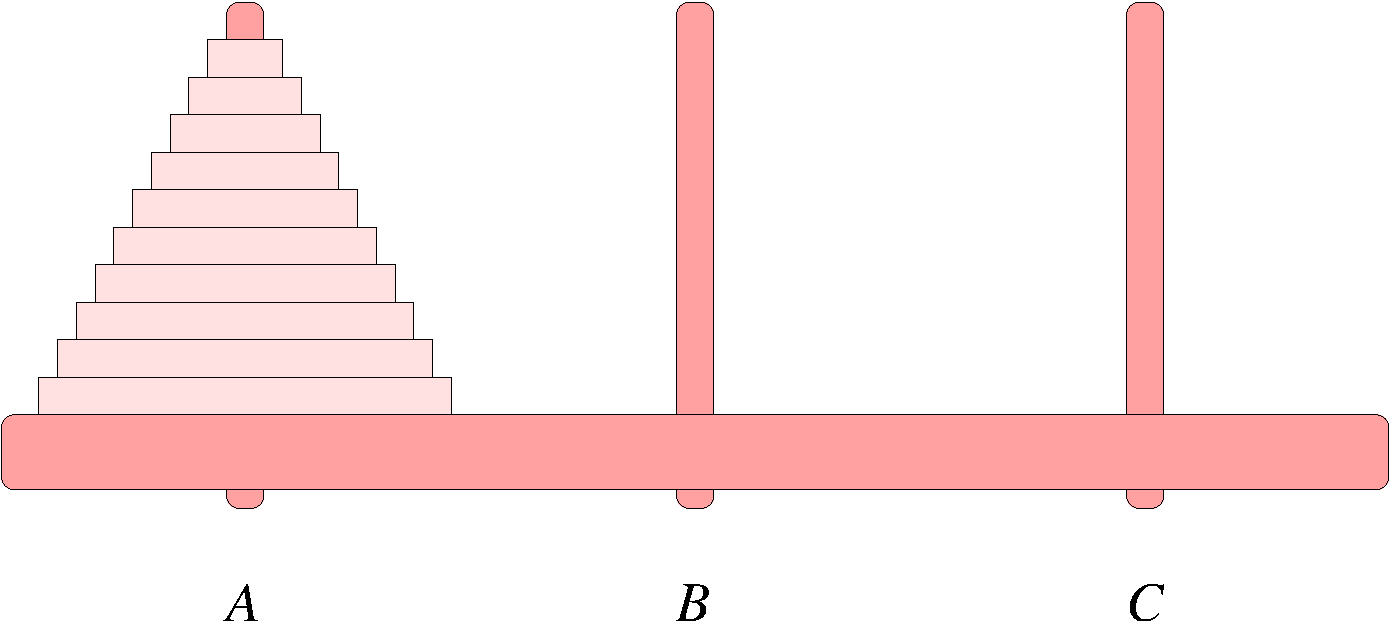
\includegraphics[height=1.5in]{towers}
    \caption{We have a sorted stack of disks at $A$ and use $B$ for temporary
    storage to move one disk at a time to $C$.
    We need $B$ to avoid any inversions among the disks.}
    \label{fig:towers}
\end{figure}
\paragraph{The Towers of Hanoi}
Recurrence relations naturally arise in the analysis of
the towers of Hanoi problem.
Here we have three pegs, $A$, $B$, $C$, and initially $n$
disks at $A$, sorted from large to small;
see \figref{towers}.
The task is to move the $n$ disks from $A$ to $C$, one by one,
without ever placing a larger disk onto a smaller disk.

\pagebreak
The following three steps solve this problem:
\begin{enumerate}
    \item % recursively move $n-1$ disks from $A$ to $B$;
    \item % move the $n$-th disk from $A$ to $C$;
    \item % recursively move $n-1$ disks from $B$ to $C$.
\end{enumerate}
When we move disks from one peg to another, we use the third
peg to help.
For the main task, we use $B$ to help.
For the first step, we exchange the roles of $B$ and $C$,
and for the third step, we exchange the roles of~$A$ and $B$.
For small instances of this problem, how many moves are needed in the algorithm
above?
\practice

In general, the number of moves is given by the solution to the
recurrence relation
\begin{eqnarray*}
    M(n)  &=&  2 M(n-1) + 1 ,
\end{eqnarray*}
with initial condition $M(0)=0$.

\begin{lemma}[Closed Form of Hanoi Problem]
    $M(n)=2^n-1$
\end{lemma}
\begin{proof}
    ~\practice
\end{proof}

\paragraph{Summary.}
Today, we introduced recurrence relations.
To find the solution, we often have to define $T(n)$
in terms of $T(n_0)$ rather than $T(n-1)$.
We also saw that different recurrences can have
the same general form.
Knowing this will help us to solve
new recurrences that are similar to others
that we have already~seen.
